\chapter*{Print NPM angka genap}
\par Kita juga dapat melakukan Print NPM yang hanya ganjil, dengan menggunakan logika modulus

\begin{enumerate}
   

\item buka spyder dan ketikan kode seperti berikut
	\begin{figure} [h]
	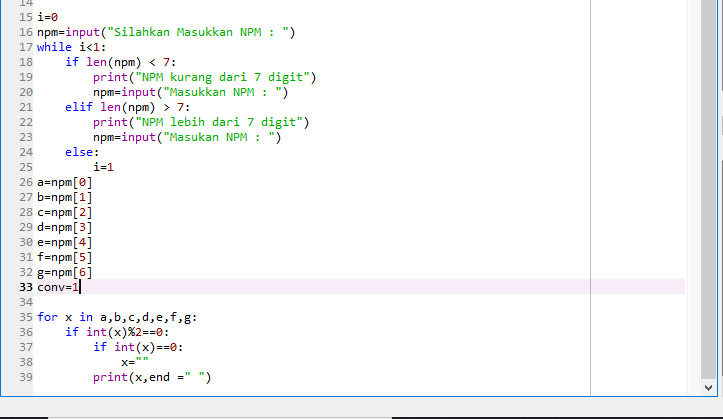
\includegraphics[width=7cm]{npm/npm5.png}
	\centering
	\end{figure}
	
	
	
 \item maka akan tercetak 
 \begin{figure} [h]
	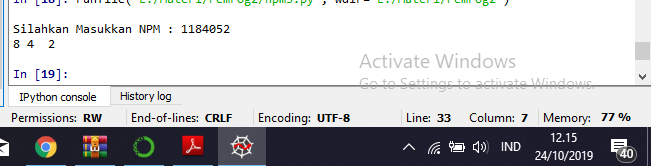
\includegraphics[width=7cm]{npm/npm6.png}
	\centering
	\end{figure}
 
	
	\end{enumerate}